\documentclass[11pt]{article}
\usepackage{csc512}

%%% For FAS
\usepackage{tikz}
\usetikzlibrary{automata, positioning, arrows}

%%%%%%%%%%%%%%%%%%%% name/id
\rfoot{\small Brian Park | 200190057}


%%%%%%%%%%%%%%%%%%%% Course/HW info
\newcommand*{\instr}{Xu Liu}
\newcommand*{\term}{Fall 2022}
\newcommand*{\coursenum}{CSC 512}
\newcommand*{\coursename}{Compiler Construction}
\newcommand*{\hwnum}{1}

\rhead{\LARGE   \fontfamily{lmdh}\selectfont	HW \hwnum}

\lfoot{\small \coursenum, \term, HW \hwnum}

%%%%%%%%%%%%%%%%%%%%%%%%%%%%%% Document Start %%%%%%%%%%%%%%%%%
\begin{document}

%%%%%%%%%%%%%%%%%%%%%%%%%%%%%%%%%%%%%%%%%%%%%%%%%%%%%%%%%%%%%%%%%%%%%%%%%%%%%%%%%%%%%%%%
% Question 1
%%%%%%%%%%%%%%%%%%%%%%%%%%%%%%%%%%%%%%%%%%%%%%%%%%%%%%%%%%%%%%%%%%%%%%%%%%%%%%%%%%%%%%%%
\section*{1}
Describe informally the languages accepted by the following \verb|FAS|:

b.
\begin{Answer}
	It only has one end state. It represents any pattern of \verb|1|s or \verb|0|s, but doesn't have a pattern for \verb|10| or \verb|01| after $s_1$ and $s_2$ which will be followed by a sequence of \verb|00| and \verb|11| respectively.
\end{Answer}

c.
\begin{Answer}
	Will contain a lot of \verb|a|'s and \verb|b|'s. Subset of \verb|aab| and \verb|baa| will appear.
\end{Answer}

\newpage

%%%%%%%%%%%%%%%%%%%%%%%%%%%%%%%%%%%%%%%%%%%%%%%%%%%%%%%%%%%%%%%%%%%%%%%%%%%%%%%%%%%%%%%%
% Question 2
%%%%%%%%%%%%%%%%%%%%%%%%%%%%%%%%%%%%%%%%%%%%%%%%%%%%%%%%%%%%%%%%%%%%%%%%%%%%%%%%%%%%%%%%
\section*{2}
Construct an \verb|FA| accepting each of the following languages: \\

b. $w \in \{0, 1\}^* | w$ contains `111' as a substring and does not contain `00' as a substring

\begin{Answer}
	\centerline{
		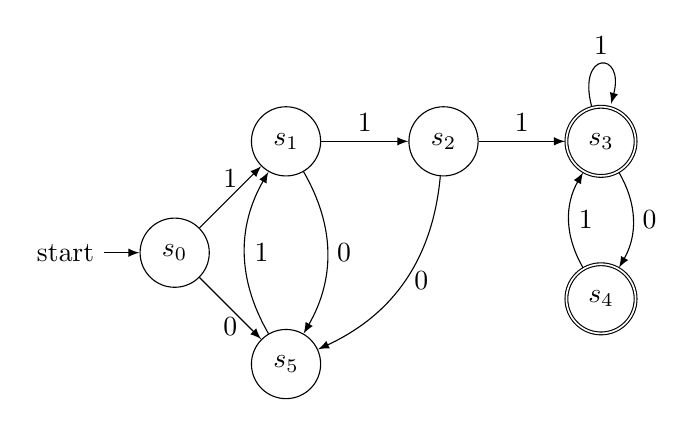
\begin{tikzpicture}[node distance = 2cm, on grid, >=latex]
			\node[state, initial] (0) {$s_0$};
			\node[state, above right of=0] (1) {$s_1$};
			\node[state, right of=1] (2) {$s_2$};
			\node[state, right of=2, accepting] (3) {$s_3$};
			\node[state, below of=3, accepting] (4) {$s_4$};
			\node[state, below right of=0] (5) {$s_5$};

			\draw[->] (0) edge[above] node{$1$} (1)
			(1) edge[below, bend left, right=0.3] node{$0$} (5)
			(5) edge[below, bend left, right=0.3] node{$1$} (1)
			(0) edge[below] node{$0$} (5)
			(1) edge[above] node{$1$} (2)
			(2) edge[below, bend left, right=0.3] node{$0$} (5)
			(2) edge[above] node{$1$} (3)
			(3) edge[loop above] node{$1$} (3)
			(3) edge[below, bend left, right=0.3] node{$0$} (4)
			(4) edge[below, bend left, right=0.3] node{$1$} (3);
		\end{tikzpicture}
	}
\end{Answer}

c. $w \in \{a, b, c\}^* | \in w$ the number of $a$'s modulo 2 is equal to the number of $b$'s modulo 3
\begin{Answer}
	\centerline{
		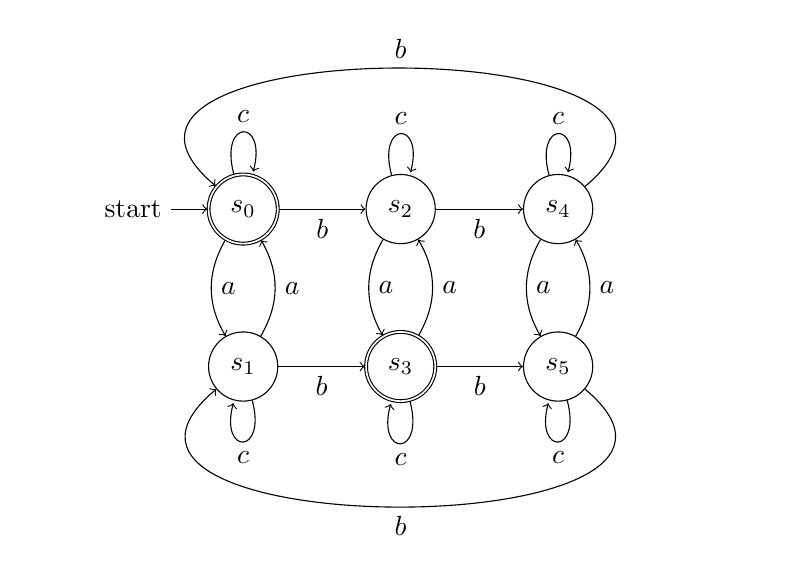
\begin{tikzpicture}[node distance = 2cm, on grid]
			\node[state, initial, accepting] (0) {$s_0$};
			\node[state, below of=0] (1) {$s_1$};
			\node[state, right of=0] (2) {$s_2$};
			\node[state, below of=2, accepting] (3) {$s_3$};
			\node[state, right of=2] (4) {$s_4$};
			\node[state, below of=4] (5) {$s_5$};

			\draw[->] (0) edge[below] node{$b$} (2)
			(2) edge[below] node{$b$} (4)
			(1) edge[below] node{$b$} (3)
			(3) edge[below] node{$b$} (5)
			(0) edge[loop above] node{$c$} (0)
			(1) edge[loop below] node{$c$} (1)
			(2) edge[loop above] node{$c$} (2)
			(3) edge[loop below] node{$c$} (3)
			(4) edge[loop above] node{$c$} (4)
			(5) edge[loop below] node{$c$} (5)
			(4) edge[above, bend right=140,looseness=1.7] node{$b$} (0)
			(5) edge[below, bend left=140,looseness=1.7] node{$b$} (1)
			(0) edge[right, bend right] node{$a$} (1)
			(2) edge[right, bend right] node{$a$} (3)
			(4) edge[right, bend right] node{$a$} (5)
			(1) edge[right, bend right] node{$a$} (0)
			(3) edge[right, bend right] node{$a$} (2)
			(5) edge[right, bend right] node{$a$} (4);

		\end{tikzpicture}
	}
\end{Answer}
\newpage

%%%%%%%%%%%%%%%%%%%%%%%%%%%%%%%%%%%%%%%%%%%%%%%%%%%%%%%%%%%%%%%%%%%%%%%%%%%%%%%%%%%%%%%%
% Question 4
%%%%%%%%%%%%%%%%%%%%%%%%%%%%%%%%%%%%%%%%%%%%%%%%%%%%%%%%%%%%%%%%%%%%%%%%%%%%%%%%%%%%%%%%
\section*{4}
Different programming languages use different notations to represent integers. Construct a regular expression for each one of the following: \\

c. Currency, in dollars, represented as a positive decimal number rounded to the nearest one-hundredth. Such numbers begin with the character \$, have commas separating each group of three digits to the left of the decimal point, and end with two digits to the right of the decimal point, for example, \$8,937.43 and \$7,777,777.77.

\begin{Answer}
	$$\$\Big([1\cdots9]([0\cdots9] | \epsilon)([0\cdots9] | \epsilon)(,[0\cdots9][0\cdots9][0\cdots9])^*\Big|0\Big).[0\cdots9][0\cdots9]$$
\end{Answer}

\newpage

%%%%%%%%%%%%%%%%%%%%%%%%%%%%%%%%%%%%%%%%%%%%%%%%%%%%%%%%%%%%%%%%%%%%%%%%%%%%%%%%%%%%%%%%
% Question 5
%%%%%%%%%%%%%%%%%%%%%%%%%%%%%%%%%%%%%%%%%%%%%%%%%%%%%%%%%%%%%%%%%%%%%%%%%%%%%%%%%%%%%%%%
\section*{5}
Write a regular expression for each of the following languages: \\

e. Given an alphabet $\Sigma = \{+, -, \times, \div, (,), \verb|id|\}$, $L$ is the set of algebraic expressions using addition, subtraction, multiplication, division, and parentheses over \verb|id|s.

\begin{Answer}
	$$L = \verb|id|(+ | - | \times | \div)\verb|id|\Big((+ | - | \times | \div)\verb|id|\Big)^*$$

	An exception is that parenthesis cannot be matched with regular expression, thus the language cannot be fully represented by regular expressions.
\end{Answer}

\newpage

%%%%%%%%%%%%%%%%%%%%%%%%%%%%%%%%%%%%%%%%%%%%%%%%%%%%%%%%%%%%%%%%%%%%%%%%%%%%%%%%%%%%%%%%
% Question 7
%%%%%%%%%%%%%%%%%%%%%%%%%%%%%%%%%%%%%%%%%%%%%%%%%%%%%%%%%%%%%%%%%%%%%%%%%%%%%%%%%%%%%%%%
\section*{7}
Consider the regular expression:
$$(01 | 10 | 00)^* 11$$

a. Use Thompson's construction to construct an NFA for RE.

\begin{Answer}
	\centerline{
		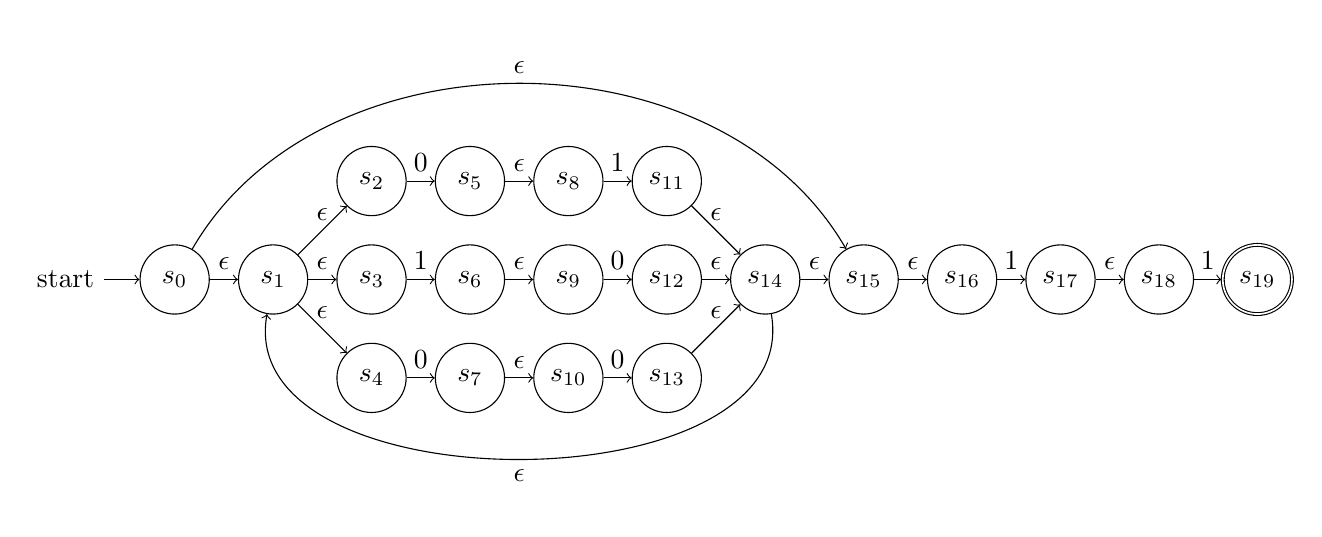
\begin{tikzpicture}[node distance = 1.25cm, on grid]
			\node[state, initial] (0) {$s_0$};
			\node[state, right of=0] (1) {$s_1$};
			\node[state, right of=1] (3) {$s_3$};
			\node[state, above of=3] (2) {$s_2$};
			\node[state, below of=3] (4) {$s_4$};
			\node[state, right of=3] (6) {$s_6$};
			\node[state, above of=6] (5) {$s_5$};
			\node[state, below of=6] (7) {$s_7$};
			\node[state, right of=6] (9) {$s_9$};
			\node[state, above of=9] (8) {$s_8$};
			\node[state, below of=9] (10) {$s_{10}$};
			\node[state, right of=9] (12) {$s_{12}$};
			\node[state, above of=12] (11) {$s_{11}$};
			\node[state, below of=12] (13) {$s_{13}$};
			\node[state, right of=12] (14) {$s_{14}$};
			\node[state, right of=14] (15) {$s_{15}$};
			\node[state, right of=15] (16) {$s_{16}$};
			\node[state, right of=16] (17) {$s_{17}$};
			\node[state, right of=17] (18) {$s_{18}$};
			\node[state, right of=18, accepting] (19) {$s_{19}$};

			\draw[->] (0) edge[above] node{$\epsilon$} (1)
			(1) edge[above] node{$\epsilon$} (2)
			(1) edge[above] node{$\epsilon$} (3)
			(1) edge[above] node{$\epsilon$} (4)

			(2) edge[above] node{$0$} (5)
			(3) edge[above] node{$1$} (6)
			(4) edge[above] node{$0$} (7)

			(5) edge[above] node{$\epsilon$} (8)
			(6) edge[above] node{$\epsilon$} (9)
			(7) edge[above] node{$\epsilon$} (10)

			(8) edge[above] node{$1$} (11)
			(9) edge[above] node{$0$} (12)
			(10) edge[above] node{$0$} (13)

			(11) edge[above] node{$\epsilon$} (14)
			(12) edge[above] node{$\epsilon$} (14)
			(13) edge[above] node{$\epsilon$} (14)

			(14) edge[above] node{$\epsilon$} (15)
			(15) edge[above] node{$\epsilon$} (16)
			(16) edge[above] node{$1$} (17)
			(17) edge[above] node{$\epsilon$} (18)
			(18) edge[above] node{$1$} (19)
			(0) edge[above, bend left=60] node{$\epsilon$} (15)
			(14) edge[below, bend left=100] node{$\epsilon$} (1);

		\end{tikzpicture}
	}
\end{Answer}

b. Convert the NFAs to DFAs.

\begin{Answer}
	\centerline{
		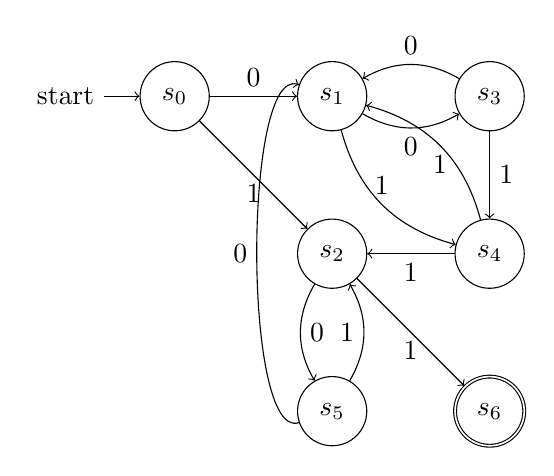
\begin{tikzpicture}[node distance = 2cm, on grid]
			\node[state, initial] (0) {$s_0$};
			\node[state, right of=0] (1) {$s_1$};
			\node[state, right of=1] (3) {$s_3$};
			\node[state, below of=1] (2) {$s_2$};
			\node[state, below of=2] (5) {$s_5$};
			\node[state, below of=3] (4) {$s_4$};
			\node[state, below of=4, accepting] (6) {$s_6$};

			\draw[->] (0) edge[above] node{$0$} (1)
			(1) edge[below, bend right] node{$0$} (3)
			(3) edge[above, bend right] node{$0$} (1)
			(3) edge[right] node{$1$} (4)
			(1) edge[above, bend right] node{$1$} (4)
			(4) edge[below, bend right] node{$1$} (1)
			(4) edge[below] node{$1$} (2)
			(2) edge[below] node{$1$} (6)
			(0) edge[below] node{$1$} (2)
			(2) edge[right, bend right] node{$0$} (5)
			(5) edge[left, bend right] node{$1$} (2)
			(5) edge[left, bend left=109, looseness=0.45] node{$0$} (1);

		\end{tikzpicture}
	}

\end{Answer}

\newpage
c. Minimize the DFAs.

\begin{Answer}
	\centerline{
		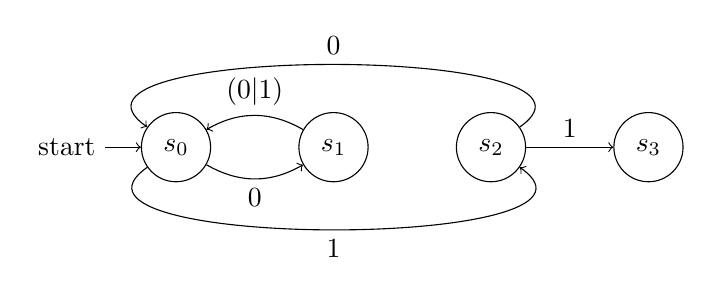
\begin{tikzpicture}[node distance = 2cm, on grid]
			\node[state, initial] (0) {$s_0$};
			\node[state, right of=0] (1) {$s_1$};
			\node[state, right of=1] (2) {$s_2$};
			\node[state, right of=2] (3) {$s_3$};


			\draw[->] (0) edge[below, bend right] node{$0$} (1)
			(1) edge[above, bend right] node{$(0|1)$} (0)
			(0) edge[below, bend right=145] node{$1$} (2)
			(2) edge[above, bend right=145] node{$0$} (0)
			(2) edge[above] node{$1$} (3);
		\end{tikzpicture}
	}
\end{Answer}

\end{document}